\documentclass[11pt,a4paper]{article}
\usepackage[utf8]{inputenc}
\usepackage[T1]{fontenc}
\usepackage[spanish,es-tabla]{babel}
\usepackage{amsmath,amssymb}
\usepackage{geometry}
\geometry{top=2.3cm,bottom=2.3cm,left=2.5cm,right=2.5cm}
\usepackage{booktabs}
\usepackage[table]{xcolor}
\usepackage{graphicx}
\usepackage{hyperref}
\usepackage{fancyhdr}
\usepackage{tcolorbox}
\usepackage{enumitem}
\usepackage{float}
\usepackage{array}
\usepackage{tikz}
\usepackage{pgfplots}
\usepackage{pdflscape}
\pgfplotsset{compat=1.18}
\usetikzlibrary{arrows.meta,calc,patterns,babel,positioning}

% Paleta institucional y estilo de planos tecnicos
\definecolor{primary}{RGB}{15,32,67}
\definecolor{secondary}{RGB}{220,53,69}
\definecolor{accent}{RGB}{0,102,204}
\definecolor{lightbg}{RGB}{245,247,250}
\definecolor{cadblue}{RGB}{24,82,145}
\definecolor{cadgrey}{RGB}{76,92,109}
\definecolor{cadorange}{RGB}{174,103,31}
\definecolor{cadgreen}{RGB}{24,123,107}
\tikzset{
  cad/.style={draw=cadblue,line width=0.75pt},
  dims/.style={<->,>=Stealth,draw=cadgrey,line width=0.55pt},
  force/.style={-{Stealth[length=2.7mm]},draw=cadorange,line width=1pt},
  support/.style={draw=cadgrey,line width=0.8pt,fill=white},
}
\hypersetup{colorlinks=true,linkcolor=accent,urlcolor=accent,bookmarks=false}
\pagestyle{empty}
\setlength{\parindent}{0pt}
\setlength{\parskip}{3.5pt}
\setlength{\emergencystretch}{3em}
\renewcommand{\arraystretch}{1.15}
\setlist[itemize]{leftmargin=*,itemsep=2pt,topsep=3pt}
\setlist[enumerate]{leftmargin=*,itemsep=3pt,topsep=3pt}
\tcbset{colback=lightbg,colframe=primary,boxrule=0.6pt,arc=1.2mm,left=3mm,right=3mm,top=2mm,bottom=2mm}

\begin{document}
\begin{center}
{\large\bfseries FASE 3: COMPORTAMIENTO INELÁSTICO DE LA COLUMNA}\\[3pt]

\end{center}
\vspace{2mm}

% --------------------------------------------------------------
% PASO 1
% --------------------------------------------------------------
\section{PASO 1: Identificación de la Pila Crítica y Datos de Entrada}

La fase 3 desarrolla el análisis no lineal de una sección circular de concreto
reforzado, con el fin de obtener su relación \textbf{momento--curvatura} bajo
una carga axial definida. 

\subsection*{Datos geométricos provenientes de la fase 2}
\begin{itemize}
  \item Puente continuo de tres tramos: $22.50\,\mathrm{m}$, $30.00\,\mathrm{m}$ y $22.50\,\mathrm{m}$; longitud total de $75.00\,\mathrm{m}$.
  \item Marco transversal integrado por dos columnas circulares.
  \item Diámetro de cada columna: $D=1.20\,\mathrm{m}$.
  \item Altura libre: $H=7.00\,\mathrm{m}$.
  \item Separación entre ejes de columnas: $S=6.00\,\mathrm{m}$.
  \item Viga cabezal: sección de $1.50\times 1.50\,\mathrm{m}$; longitud de $9.60\,\mathrm{m}$.
  \item Carga axial permanente en la base de la columna: $P_{c,\mathrm{perm}}=1{,}928.92\,\mathrm{kN}$.
  \item Reacción vehicular HL-93 considerada para la columna crítica: $P_{LL}=595.82\,\mathrm{kN}$.
\end{itemize}

\begin{figure}[H]
\centering
\resizebox{0.75\linewidth}{!}{%
\begin{tikzpicture}[x=1.13cm,y=0.67cm,font=\footnotesize]
  % viga cabezal
  \fill[cadblue!9] (0,7.00) rectangle (9.6,8.5);
  \draw[cad,line width=1.15pt] (0,7.00) rectangle (9.6,8.5);
  % columnas, ejes
  \foreach \x in {1.8,7.8}{
    \fill[cadblue!15] (\x-.36,0) rectangle (\x+.36,7.0);
    \draw[cad,line width=1.05pt] (\x-.36,0) rectangle (\x+.36,7.0);
    \draw[cadgrey,dash pattern=on 2pt off 2pt] (\x,-.2)--(\x,8.7);
    \draw[support] (\x-.55,-.27) rectangle (\x+.55,-.05);
    \foreach \i in {-2,-1,0,1,2}{\draw[cadgrey,thin] (\x+\i*.2-.10,-.39)--(\x+\i*.2,-.27);}
  }
  % cotas horizontal y vertical
  \draw[cadgrey,thin] (1.8,8.8)--(1.8,9.35);
  \draw[cadgrey,thin] (7.8,8.8)--(7.8,9.35);
  \draw[dims] (1.8,9.18)--(7.8,9.18) node[midway,above] {$6.00\,\mathrm{m}$};
  \draw[cadgrey,thin] (0,-.65)--(0,-1.3);
  \draw[cadgrey,thin] (9.6,-.65)--(9.6,-1.3);
  \draw[dims] (0,-1.08)--(9.6,-1.08) node[midway,below] {Cabezal $9.60\,\mathrm{m}$};
  \draw[cadgrey,thin] (0.6,0)--(.32,0);
  \draw[cadgrey,thin] (.6,7)--(.32,7);
  \draw[dims] (.42,0)--(.42,7) node[midway,left] {$H=7.00\,\mathrm{m}$};
  \draw[force] (1.8,10.8)--(1.8,8.62);
  \draw[force] (7.8,10.8)--(7.8,8.62);
  \node[above,cadorange] at (4.8,10.8) {Cargas gravitacionales transmitidas al pórtico};
  \node[below,cadblue] at (1.8,-.44) {C1};
  \node[below,cadblue] at (7.8,-.44) {C2};
  \node[cadgrey] at (4.8,7.76) {Viga cabezal $1.50\times1.50\,\mathrm{m}$};
  \node[cadgrey] at (4.8,3.7) {Columnas $D=1.20\,\mathrm{m}$};
\end{tikzpicture}}
\caption{Esquema del pórtico transversal. Cotas en metros; representación de análisis, no plano de construcción.}
\end{figure}

\subsection*{Carga axial del caso sísmico adoptado}
En la fase 2 se estableció una participación vehicular sísmica de
$\gamma_{EQ}=0.50$. La carga axial de la columna crítica se integra así:
\begin{equation*}
P_c=P_{c,\mathrm{perm}}+\gamma_{EQ}P_{LL}
\end{equation*}
\begin{equation*}
P_c=1{,}928.92+0.50(595.82)
\end{equation*}
\begin{equation*}
\boxed{P_c=2{,}226.83\,\mathrm{kN}}
\end{equation*}


\subsection*{Alcance de la carga axial}

$P_c$ corresponde a la carga axial de cálculo en la base de la columna crítica dentro del procedimiento de la fase 2. El valor HL-93 procede del reparto longitudinal y transversal allí desarrollado.



% --------------------------------------------------------------
% PASO 2
% --------------------------------------------------------------
\section{PASO 2: Propiedades Mecánicas de los Materiales}

\subsection{Resistencia nominal y esperada del concreto}
Se conserva el criterio de materiales utilizado en el laboratorio del curso:
\begin{equation*}
f'_{ce}=1.30f'_c
\end{equation*}
\begin{equation*}
f'_{ce}=1.30(4{,}000\,\mathrm{psi})=\boxed{5{,}200\,\mathrm{psi}}
\end{equation*}
Con $1\,\mathrm{psi}=0.006894757\,\mathrm{MPa}$:
\begin{align*}
f'_c&=4{,}000(0.006894757)=27.58\,\mathrm{MPa},\\
f'_{ce}&=5{,}200(0.006894757)=35.85\,\mathrm{MPa}.
\end{align*}

\subsection{Resistencia nominal y esperada del acero}
Para acero longitudinal de Grado 60 se utiliza la resistencia esperada
indicada en la guía de SAP2000:
\begin{equation*}
f_{ye}=1.10f_y=1.10(60\,\mathrm{ksi})=\boxed{66\,\mathrm{ksi}}
\end{equation*}
Con $1\,\mathrm{ksi}=6.894757\,\mathrm{MPa}$:
\begin{align*}
f_y&=413.69\,\mathrm{MPa},\\
f_{ye}&=455.05\,\mathrm{MPa}.
\end{align*}

\begin{table}[H]
\centering
\caption{Resumen de materiales adoptados para el análisis no lineal.}
\begin{tabular}{p{8.0cm}r l}
\toprule
\textbf{Parámetro} & \textbf{Valor} & \textbf{Unidad}\\
\midrule
Resistencia nominal del concreto $f'_c$ & 4,000 & psi\\
Resistencia esperada del concreto $f'_{ce}$ & 5,200 & psi\\
Fluencia nominal del acero $f_y$ & 60 & ksi\\
Fluencia esperada del acero $f_{ye}$ & 66 & ksi\\
Modelo del concreto del núcleo & \multicolumn{2}{l}{Mander Confined}\\
\bottomrule
\end{tabular}
\end{table}



% --------------------------------------------------------------
% PASO 3
% --------------------------------------------------------------
\section{PASO 3: Geometría y Propiedades de la Sección Circular}

\subsection{Área bruta de la sección ($A_g$)}
\begin{equation*}
A_g=\frac{\pi D^2}{4}
\end{equation*}
\begin{equation*}
A_g=\frac{\pi(1.20\,\mathrm{m})^2}{4}
\end{equation*}
\begin{equation*}
\boxed{A_g=1.13097\,\mathrm{m}^2=1{,}130{,}973.36\,\mathrm{mm}^2}
\end{equation*}

\subsection{Momento de inercia bruto ($I_g$)}
Para una sección circular maciza:
\begin{equation*}
I_g=\frac{\pi D^4}{64}
  =\frac{\pi(1.20\,\mathrm{m})^4}{64}
  =\boxed{0.10179\,\mathrm{m}^4}
\end{equation*}

\subsection{Módulo resistente geométrico ($S_g$)}
\begin{equation*}
S_g=\frac{I_g}{D/2}=\frac{\pi D^3}{32}
=\frac{\pi(1.20)^3}{32}
=\boxed{0.16965\,\mathrm{m}^3}
\end{equation*}

Estas son propiedades \textbf{brutas} de la geometría; no representan por sí
mismas la rigidez agrietada ni la capacidad inelástica de la columna.

\subsection{Conversión a pulgadas para SAP2000}
\begin{align*}
D&=1.20(39.370079)=\boxed{47.244\,\mathrm{in}},\\
H&=7.00(39.370079)=\boxed{275.591\,\mathrm{in}},\\
S&=6.00(39.370079)=\boxed{236.220\,\mathrm{in}},\\
b_{\mathrm{cabezal}}=h_{\mathrm{cabezal}}&=1.50(39.370079)=\boxed{59.055\,\mathrm{in}}.
\end{align*}

% --------------------------------------------------------------
% PASO 4
% --------------------------------------------------------------
\section{PASO 4: Refuerzo Longitudinal y Cuantía Geométrica}

El armado utilizado para el análisis de la sección está compuesto por
$26$ barras longitudinales No.~14, distribuidas regularmente alrededor
del perímetro de la columna circular.

\subsection{Área total de acero longitudinal ($A_s$)}
\begin{align*}
n&=26\ \text{barras},\\
A_b&=2.25\,\mathrm{in}^2/\text{barra},\\
A_s&=n A_b=26(2.25)=58.50\,\mathrm{in}^2.
\end{align*}
Con $1\,\mathrm{in}^2=645.16\,\mathrm{mm}^2$:
\begin{equation*}
A_s=58.50(645.16)=\boxed{37{,}741.86\,\mathrm{mm}^2}
\end{equation*}

\subsection{Cuantía longitudinal ($\rho_l$)}
\begin{equation*}
\rho_l=\frac{A_s}{A_g}\times100\%
\end{equation*}
\begin{equation*}
\rho_l=\frac{37{,}741.86}{1{,}130{,}973.36}\times100\%
  =\boxed{3.34\%}
\end{equation*}


\begin{figure}[H]
\centering
\begin{tikzpicture}[scale=0.86,font=\footnotesize]
  \fill[cadblue!5] (0,0) circle (2.75);
  \draw[cad,line width=1.15pt] (0,0) circle (2.75);
  \draw[cadgreen,line width=1.1pt] (0,0) circle (2.46);
  \foreach \i in {0,...,25}{
     \pgfmathsetmacro{\ang}{90+360*\i/26}
     \fill[primary] (\ang:2.40) circle (0.098);
  }
  \draw[dims] (-2.75,-3.2)--(2.75,-3.2)
    node[midway,below] {$D=1.20\,\mathrm{m}$};
  \draw[cadgrey,thin] (-2.75,-2.7)--(-2.75,-3.42);
  \draw[cadgrey,thin] (2.75,-2.7)--(2.75,-3.42);
  \draw[cadgrey,thin] (1.80,1.44)--(3.50,2.0);
  \node[anchor=west,cadblue] at (3.55,2.0) {Concreto de la sección};
  \draw[cadgrey,thin] (1.15,-1.95)--(3.52,-1.25);
  \node[anchor=west,primary] at (3.57,-1.25) {26 barras No.~14};
  \draw[cadgrey,thin] (-2.27,1.04)--(-3.7,1.65);
  \node[anchor=east,cadgreen] at (-3.73,1.65) {Aro No.~8};
  \node[cadgrey] at (0,-4.10) {Croquis de armado; geometría del núcleo revisada en Section Designer.};
\end{tikzpicture}
\caption{Configuración circular de refuerzo longitudinal y confinamiento para Section Designer.}
\end{figure}

% --------------------------------------------------------------
% PASO 5
% --------------------------------------------------------------
\section{PASO 5: Refuerzo Transversal y Confinamiento}

La sección modelada emplea aros No.~8 con separación longitudinal de
$5\,\mathrm{in}$. El recubrimiento \textbf{libre hasta la cara exterior
del aro} es de $2\,\mathrm{in}$. 

\subsection{Datos del confinamiento}
\begin{align*}
d_h&=1.00\,\mathrm{in}=\boxed{25.40\,\mathrm{mm}},\\
s&=5.00\,\mathrm{in}=\boxed{127.00\,\mathrm{mm}},\\
c&=2.00\,\mathrm{in}=\boxed{50.80\,\mathrm{mm}}.
\end{align*}

\subsection{Posición del aro y recubrimiento verificados en SAP2000}


Para el aro No.~8 se utiliza el diámetro nominal $d_h=1.00\,\mathrm{in}$.
El recubrimiento libre al exterior de dicho aro se comprueba mediante:
\begin{equation*}
c_{\mathrm{libre}}=\frac{D-D_{h,\mathrm{CL}}}{2}-\frac{d_h}{2}
\end{equation*}
\begin{equation*}
c_{\mathrm{libre}}=\frac{47.244-42.244}{2}-\frac{1.00}{2}
=\boxed{2.00\,\mathrm{in}=50.8\,\mathrm{mm}}
\end{equation*}
La misma geometría implica:
\begin{align*}
D_{h,\mathrm{CL}} &= 42.244\,\mathrm{in}=1{,}072.9976\,\mathrm{mm},\\
D_{\mathrm{int,aro}} &=42.244-1.00
=\boxed{41.244\,\mathrm{in}}.
\end{align*}


\subsection{Cuantía volumétrica geométrica aproximada}
Considerando el área nominal del aro No.~8 de
$A_h=0.79\,\mathrm{in}^2$, se calcula un indicador geométrico:
\begin{equation*}
\rho_s\approx\frac{4A_h}{sD_{h,\mathrm{CL}}}
=\frac{4(0.79)}{5(42.244)}
=\boxed{0.01496\approx 1.50\%}
\end{equation*}

\subsection{Respuesta constitutiva del concreto confinado}
La configuración mostrada por SAP2000 utiliza
\textit{Mander-Confined(C)}, tipo \texttt{Hoop}, aros No.~8
cada $5\,\mathrm{in}$, $26$ barras longitudinales y acero transversal
con $f_{yh}=60\,\mathrm{ksi}$.
En la gráfica constitutiva se observa una resistencia confinada máxima
aproximada $f'_{cc}\simeq7.7\,\mathrm{ksi}$, frente a la resistencia
base $f'_{ce}=5.2\,\mathrm{ksi}$. Las deformaciones de la ventana
constitutiva son parámetros del material; no deben confundirse con
las curvaturas de falla de la sección.


\begin{figure}[H]
  \centering
  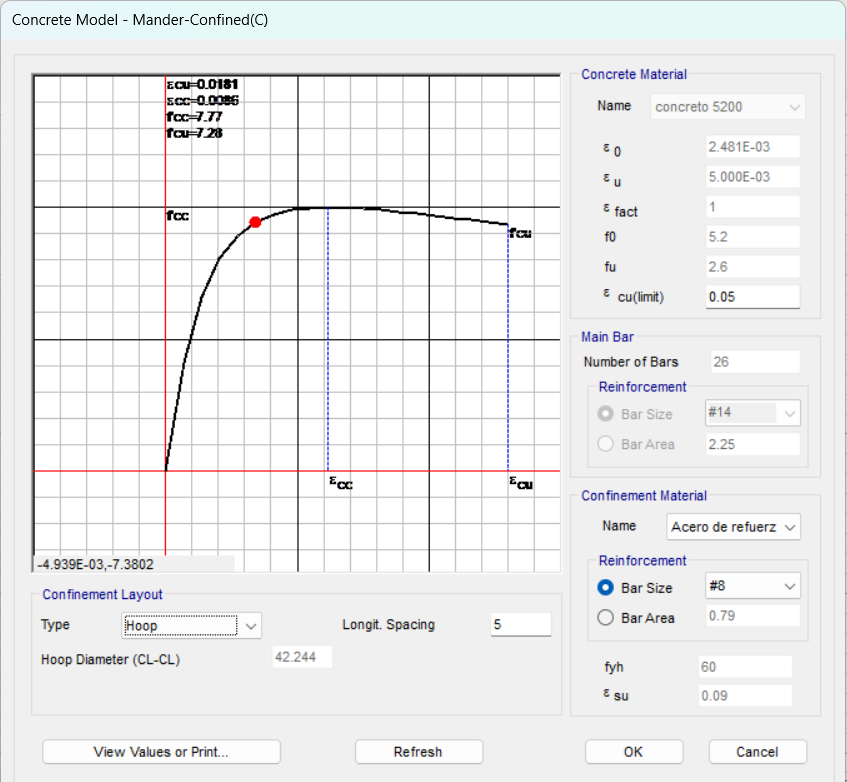
\includegraphics[width=0.82\linewidth,height=0.56\textheight,keepaspectratio]{figuras_sap/sap_modelo_mander_real.png}
  \caption{Captura original de SAP2000: modelo de concreto confinado de Mander para la sección circular, con aros No.~8 cada 5 pulgadas y 26 barras longitudinales.}
  \label{fig:sap-mander-original}
\end{figure}

\subsection{Relación geométrica de separación}
\begin{equation*}
\frac{s}{D}=\frac{127}{1{,}200}=\boxed{0.1058}
\end{equation*}


\begin{figure}[H]
\centering
\begin{tikzpicture}[x=1.0cm,y=1.0cm,font=\footnotesize]
\fill[cadblue!5] (1,0) rectangle (4,5.0);
\draw[cad,line width=1pt] (1,0) rectangle (4,5.0);
\foreach \x in {1.48,2.15,2.85,3.52}{
  \draw[primary,line width=2.1pt] (\x,.08)--(\x,4.92);
}
\foreach \y in {.4,1.15,1.9,2.65,3.4,4.15,4.9}{
  \draw[cadgreen,line width=1.1pt] (1.10,\y)--(3.90,\y);
}
\draw[dims] (4.4,1.15)--(4.4,1.90) node[midway,right] {$s=127\,\mathrm{mm}$};
\node[anchor=west,cadblue] at (5.1,4.48) {Concreto de la columna};
\node[anchor=west,primary] at (5.1,3.35) {Barras longitudinales No.~14};
\node[anchor=west,cadgreen] at (5.1,2.20) {Aros transversales No.~8};
\node[anchor=west,cadgrey] at (5.1,.65) {Vista esquemática, sin escala};
\end{tikzpicture}
\caption{Disposición longitudinal del acero de confinamiento. La forma y anclaje de los aros requieren revisión de detallado.}
\end{figure}

% --------------------------------------------------------------
% PASO 6
% --------------------------------------------------------------
\section{PASO 6: Carga Axial y Conversión de Unidades para SAP2000}

\subsection{Integración de la carga axial}
Según la fase 2, la carga permanente se obtiene de la carga en el tope
más el peso propio de la columna:
\begin{equation*}
P_{c,\mathrm{perm}}=1{,}738.92+190.00
=1{,}928.92\,\mathrm{kN}
\end{equation*}
La contribución sísmica adoptada de la carga viva es:
\begin{equation*}
P_{LL,\mathrm{sismo}}=\gamma_{EQ}P_{LL}
=0.50(595.82)=\boxed{297.91\,\mathrm{kN}}
\end{equation*}
Por tanto:
\begin{equation*}
P_c=1{,}928.92+297.91=\boxed{2{,}226.83\,\mathrm{kN}}
\end{equation*}

\subsection{Conversión de $\mathrm{kN}$ a $\mathrm{kip}$}
Con $1\,\mathrm{kip}=4.4482216\,\mathrm{kN}$:
\begin{equation*}
P_c=\frac{2{,}226.83}{4.4482216}
=\boxed{500.61\,\mathrm{kip}}
\end{equation*}

\subsection{Comprobación de esfuerzo axial promedio}
Como comprobación de orden de magnitud, el esfuerzo axial promedio
respecto del área bruta es:
\begin{equation*}
\sigma_{\mathrm{prom}}=\frac{P_c}{A_g}
=\frac{2{,}226.83\,\mathrm{kN}}{1.13097\,\mathrm{m}^2}
=\boxed{1.97\,\mathrm{MPa}}
\end{equation*}
Este promedio no representa la distribución real de esfuerzos en una
sección sometida simultáneamente a carga axial y flexión, ni una
comprobación de capacidad resistente.





% --------------------------------------------------------------
% PASO 7
% --------------------------------------------------------------
\section{PASO 7: Procedimiento de Modelación No Lineal en SAP2000}

\subsection{Definición del material}

\begin{figure}[H]
  \centering
  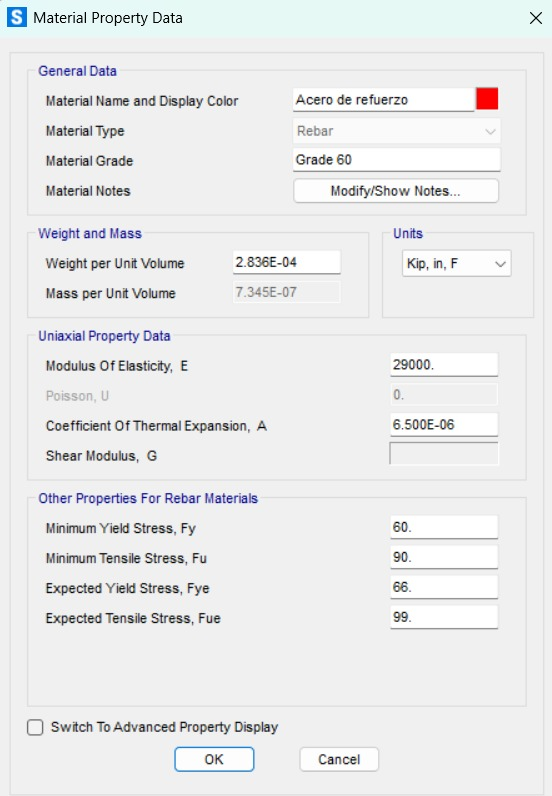
\includegraphics[width=0.82\linewidth,height=0.56\textheight,keepaspectratio]{figuras_sap/materiales.png}
  \caption{Captura original de SAP2000: Definiendo materiales.}
  \label{fig:sap-mander-original}
\end{figure}



\subsection{Definición de la sección en Section Designer}


\begin{figure}[H]
  \centering
  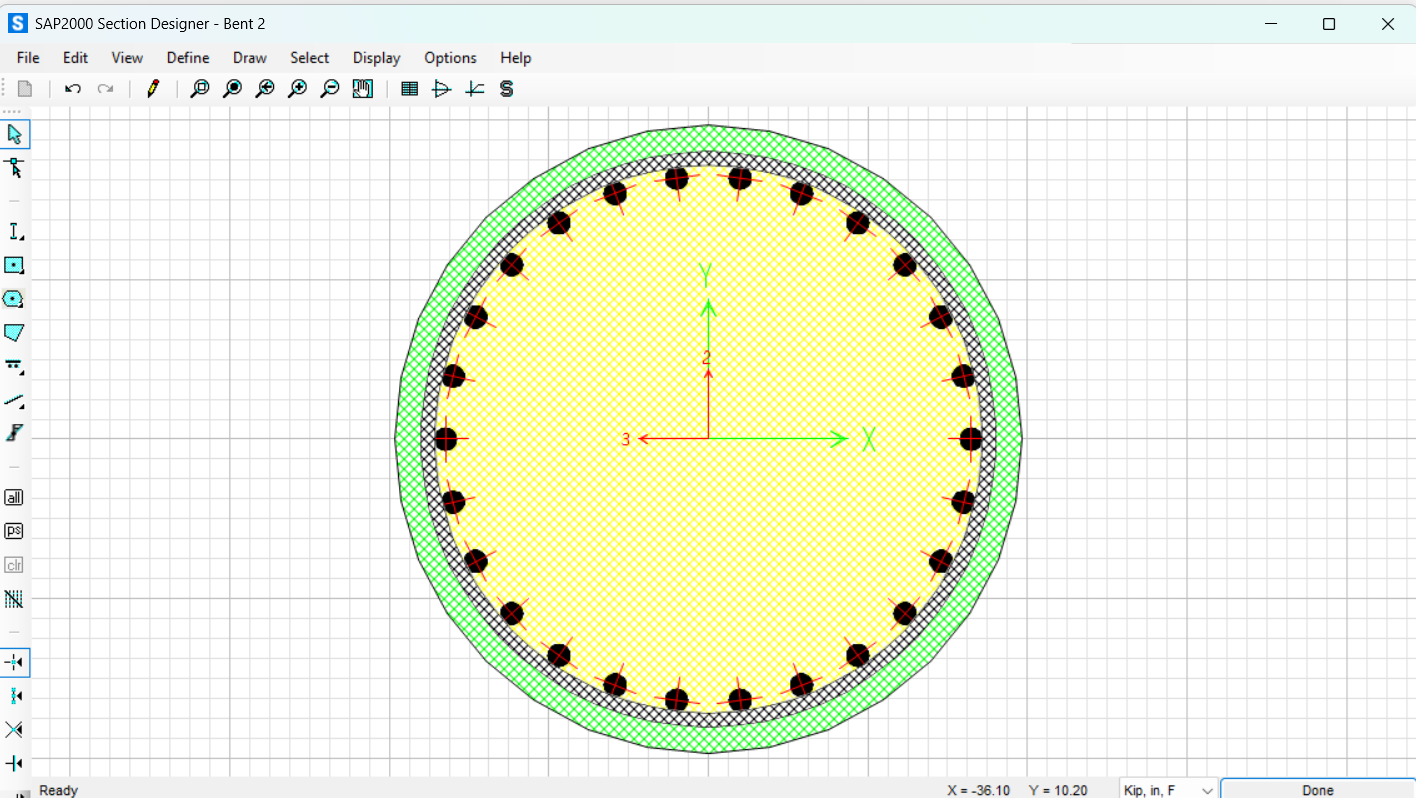
\includegraphics[width=0.85\linewidth,height=0.56\textheight,keepaspectratio]{figuras_sap/CIRCULO.png}
  \caption{Captura original de SAP2000}
  \label{fig:sap-mander-original}
\end{figure}


\subsection{Generación del diagrama momento--curvatura}


\begin{table}[H]
\centering
\small
\caption{Configuración utilizada para el diagrama momento--curvatura.}
\begin{tabular}{p{8.8cm}p{4.5cm}}
\toprule
\textbf{Parámetro} & \textbf{Configuración comprobada}\\
\midrule
Diámetro de columna & $47.244\,\mathrm{in}$\\
Armadura longitudinal & 26 barras No.~14\\
Aros & No.~8 @ $5\,\mathrm{in}$\\
Diámetro del aro (eje a eje) & $42.244\,\mathrm{in}$\\
Recubrimiento libre al aro & $2.00\,\mathrm{in}$\\
Resistencias del acero $f_y/f_{ye}$ & $60/66\,\mathrm{ksi}$\\
Modelo de concreto & Mander-Confined(C)\\
Carga axial $P$ & $-500.61\,\mathrm{kip}$\\
Ángulo de flexión & $0^\circ$\\
Idealización & Caltrans, activada\\
Puntos del análisis & $20$\\
\bottomrule
\end{tabular}
\end{table}



% --------------------------------------------------------------

\begin{figure}[H]
  \centering
  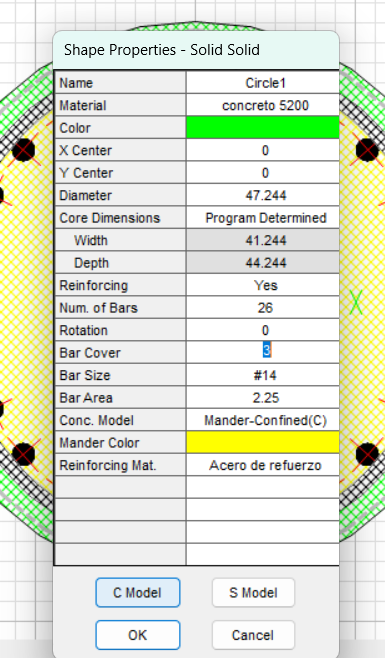
\includegraphics[width=0.45\linewidth,height=0.48\textheight,keepaspectratio]{figuras_sap/sap_seccion_real.png}
  \caption{Captura original de las propiedades de la sección circular en SAP2000, con diámetro de 47.244 pulgadas, recubrimiento de barras configurado en 3 pulgadas y 26 barras No.~14.}
  \label{fig:sap-seccion-original}
\end{figure}

\begin{figure}[H]
  \centering
  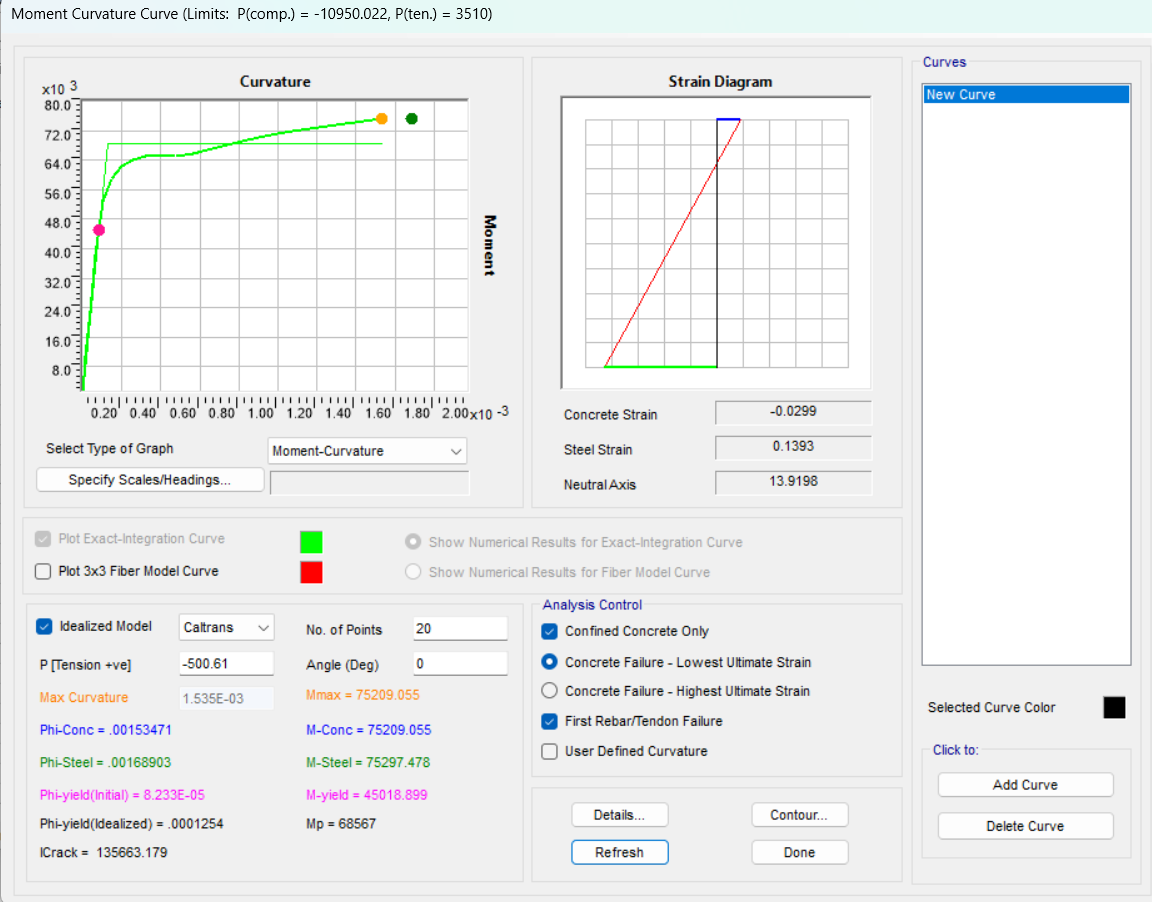
\includegraphics[width=0.93\linewidth,height=0.72\textheight,keepaspectratio]{figuras_sap/sap_configuracion_curva_real.png}
  \caption{Captura original de la ventana \textit{Moment Curvature Curve}, con carga axial $P=-500.61\,\mathrm{kip}$, idealización \textit{Caltrans} y resultados de la sección corregida.}
  \label{fig:sap-ventana-curva-original}
\end{figure}

% --------------------------------------------------------------
% PASO 8
% --------------------------------------------------------------
\section{PASO 8: Diagrama Momento--Curvatura Obtenido de SAP2000}

\subsection{Resultado de la integración no lineal de la sección}
La curva obtenida en \textit{Section Designer} corresponde a la carga
axial de compresión $P=-500.61\,\mathrm{kip}$ y a la geometría
corregida del refuerzo transversal. En el reporte de SAP2000 las unidades
activas son \texttt{Kip, in, F}; por tanto, el momento se expresa en
$\mathrm{kip\,in}$ y la curvatura en $\mathrm{in}^{-1}$.


\begin{figure}[H]
  \centering
  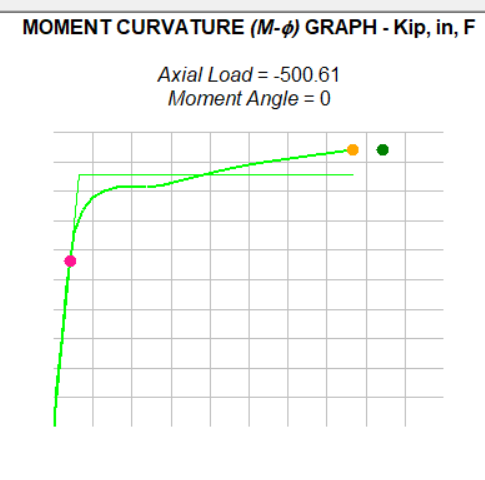
\includegraphics[width=0.85\linewidth,height=0.54\textheight,keepaspectratio]{figuras_sap/sap_curva_recorte_original.png}
  \caption{Recorte de la gráfica original del reporte de SAP2000 para la relación momento--curvatura, con carga axial de $-500.61\,\mathrm{kip}$ e idealización \textit{Caltrans}. La captura íntegra del reporte se conserva en el proyecto Overleaf.}
  \label{fig:sap-reporte-momento-curvatura-original}
\end{figure}


\subsection{Tabla de los 20 puntos de la curva}




Esta tabla Contiene los esfuerzos, las deformaciones, las fuerzas internas, las curvaturas y los momentos de los 20 puntos del análisis realizado con $P=-500.61\,\mathrm{kip}$.


\begin{center}
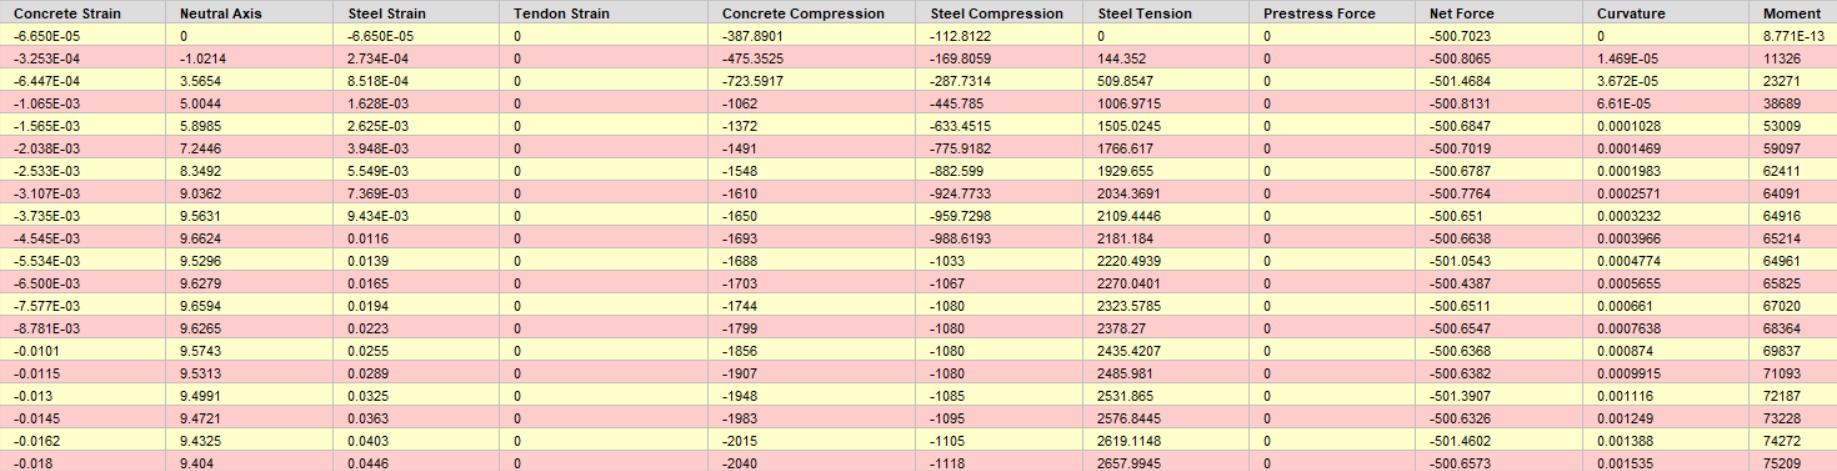
\includegraphics[width=0.99\linewidth,height=0.90\textheight,keepaspectratio]{figuras_sap/sap_tabla_integracion_real.png}
\end{center}
\begin{center}
\small\textit{}
\end{center}

La tabla siguiente transcribe los valores de curvatura y momento
proporcionados por la salida de integración exacta de SAP2000.

\begin{table}[H]
\centering
\small
\caption{Datos numéricos de momento--curvatura: sección circular corregida.}
\setlength{\tabcolsep}{6pt}
\begin{tabular}{r r r r}
\toprule
\textbf{Punto} & \textbf{$\phi$ ($\mathrm{in}^{-1}$)} &
\textbf{$M$ ($\mathrm{kip\,in}$)} & \textbf{Observación}\\
\midrule
 1 & 0             & 0      & Inicio\\
 2 & $1.469\times10^{-5}$ & 11,326 & \\
 3 & $3.672\times10^{-5}$ & 23,271 & \\
 4 & $6.615\times10^{-5}$ & 38,689 & \\
 5 & $1.028\times10^{-4}$ & 53,009 & \\
 6 & $1.469\times10^{-4}$ & 59,097 & \\
 7 & $1.983\times10^{-4}$ & 62,411 & \\
 8 & $2.571\times10^{-4}$ & 64,091 & \\
 9 & $3.232\times10^{-4}$ & 64,916 & \\
10 & $3.966\times10^{-4}$ & 65,214 & \\
11 & $4.774\times10^{-4}$ & 64,961 & \\
12 & $5.655\times10^{-4}$ & 65,825 & \\
13 & $6.610\times10^{-4}$ & 67,020 & \\
14 & $7.638\times10^{-4}$ & 68,364 & \\
15 & $8.740\times10^{-4}$ & 69,837 & \\
16 & $9.915\times10^{-4}$ & 71,093 & \\
17 & $1.116\times10^{-3}$ & 72,187 & \\
18 & $1.249\times10^{-3}$ & 73,228 & \\
19 & $1.388\times10^{-3}$ & 74,272 & \\
20 & $1.535\times10^{-3}$ & 75,209 & Límite\\
\bottomrule
\end{tabular}
\end{table}

La fuerza axial tabulada permanece aproximadamente entre
$-501.47$ y $-500.44\,\mathrm{kip}$; las pequeñas variaciones
corresponden al procedimiento numérico de integración. El último punto
coincide, con el redondeo de impresión, con el límite de concreto de
$\phi_{\mathrm{conc}}=1.53471\times10^{-3}\,\mathrm{in}^{-1}$.

\subsection{Resultados característicos del reporte}
\begin{table}[H]
\centering
\small
\caption{Parámetros de la respuesta no lineal reportados por SAP2000.}
\begin{tabular}{p{8.5cm}r l}
\toprule
\textbf{Resultado} & \textbf{Valor} & \textbf{Unidad}\\
\midrule
Momento de primera fluencia $M_y$ & 45,019 & $\mathrm{kip\,in}$\\
Curvatura de primera fluencia $\phi_{y,\mathrm{ini}}$ & $8.233\times10^{-5}$ & $\mathrm{in}^{-1}$\\
Curvatura de fluencia idealizada $\phi_{y,\mathrm{id}}$ & $1.254\times10^{-4}$ & $\mathrm{in}^{-1}$\\
Momento plástico idealizado $M_p$ & \textbf{68,567} & $\mathrm{kip\,in}$\\
Curvatura límite del concreto $\phi_{\mathrm{conc}}$ & $1.53471\times10^{-3}$ & $\mathrm{in}^{-1}$\\
Momento al límite del concreto $M_{\mathrm{conc}}$ & 75,209.055 & $\mathrm{kip\,in}$\\
Curvatura límite del acero $\phi_{\mathrm{steel}}$ & $1.68903\times10^{-3}$ & $\mathrm{in}^{-1}$\\
Momento al límite del acero $M_{\mathrm{steel}}$ & 75,297.478 & $\mathrm{kip\,in}$\\
\bottomrule
\end{tabular}
\end{table}


\begin{figure}[H]
  \centering
  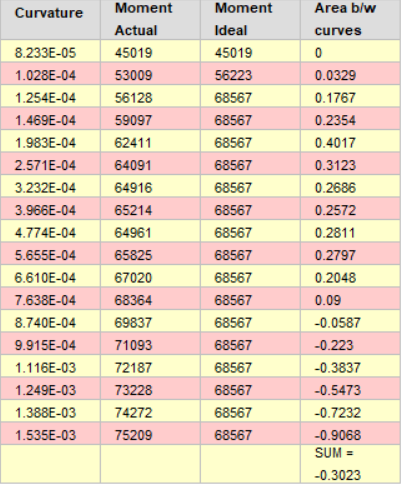
\includegraphics[width=0.63\linewidth,height=0.48\textheight,keepaspectratio]{figuras_sap/sap_tabla_idealizacion_real.png}
  \caption{Tabla original exportada de SAP2000: idealización \textit{Caltrans} y diferencias de áreas entre la curva real y la curva idealizada.}
  \label{fig:sap-tabla-caltrans-original}
\end{figure}



% --------------------------------------------------------------
% PASO 9
% --------------------------------------------------------------
\section{PASO 9: Momento Plástico, Fluencia y Ductilidad de Curvatura}

\subsection{Momento plástico idealizado de la sección}
Se adopta como momento plástico el valor del modelo idealizado
\textit{Caltrans}, calculado por SAP2000 para la carga axial y el armado
verificados:
\begin{equation*}
\boxed{M_p=68{,}567\,\mathrm{kip\,in}}
\end{equation*}
El momento plástico idealizado se diferencia del momento al límite del
concreto $M_{\mathrm{conc}}=75{,}209.055\,\mathrm{kip\,in}$:
son parámetros de la misma respuesta con definiciones distintas.

\subsection{Conversión del momento a unidades SI}
Con $1\,\mathrm{kip}=4.4482216\,\mathrm{kN}$ y
$1\,\mathrm{in}=0.0254\,\mathrm{m}$:
\begin{equation*}
1\,\mathrm{kip\,in}=4.4482216(0.0254)
=0.11298483\,\mathrm{kN\,m}
\end{equation*}
\begin{align*}
M_y &=45{,}019(0.11298483)
      =\boxed{5{,}086.46\,\mathrm{kN\,m}},\\[2pt]
M_p &=68{,}567(0.11298483)
      =\boxed{7{,}747.03\,\mathrm{kN\,m}},\\[2pt]
M_{\mathrm{conc}}&=75{,}209.055(0.11298483)
      =\boxed{8{,}497.48\,\mathrm{kN\,m}}.
\end{align*}

\subsection{Curvaturas equivalentes en el sistema SI}
La curvatura tiene dimensiones de longitud inversa; por consiguiente,
para convertir $\mathrm{in}^{-1}$ a $\mathrm{m}^{-1}$ se divide entre
$0.0254$:
\begin{align*}
\phi_{y,\mathrm{ini}}&=\frac{8.233\times10^{-5}}{0.0254}
  =0.0032413\,\mathrm{m}^{-1},\\
\phi_{y,\mathrm{id}}&=\frac{1.254\times10^{-4}}{0.0254}
  =0.0049370\,\mathrm{m}^{-1},\\
\phi_{u}&=\phi_{\mathrm{conc}}=
\frac{1.53471\times10^{-3}}{0.0254}
  =0.0604217\,\mathrm{m}^{-1}.
\end{align*}

\subsection{Cálculo de ductilidad de curvatura}
La ductilidad de curvatura de la sección se obtiene con la curvatura
límite seleccionada y la curvatura de fluencia \emph{idealizada}:
\begin{equation*}
\mu_{\phi}=\frac{\phi_{u}}{\phi_{y,\mathrm{id}}}
\end{equation*}
\begin{equation*}
\mu_{\phi}=\frac{0.00153471}{0.0001254}
=\boxed{12.24}
\end{equation*}
La ductilidad \emph{de curvatura} no se interpreta como ductilidad
lateral o global del pórtico. Su valor depende del criterio de fin de
curva seleccionado en Section Designer y de la idealización de fluencia.

\subsection{Comparación entre el momento idealizado y el límite del concreto}
\begin{equation*}
\frac{M_{\mathrm{conc}}}{M_p}
=\frac{75{,}209.055}{68{,}567}
=\boxed{1.097}
\end{equation*}
El cociente anterior caracteriza la diferencia entre dos puntos del
reporte. No es un factor normativo de sobrerresistencia y no sustituye
las verificaciones de diseño por capacidad.

\begin{tcolorbox}[title={Resultados consolidados de la fase 3}]
\begin{align*}
P&=-500.61\,\mathrm{kip},\\
M_y&=45{,}019\,\mathrm{kip\,in},\\
M_p&=\boxed{68{,}567\,\mathrm{kip\,in}}
     =\boxed{7{,}747.03\,\mathrm{kN\,m}},\\
\phi_{y,\mathrm{id}}&=1.254\times10^{-4}\,\mathrm{in}^{-1},\\
\phi_u&=1.53471\times10^{-3}\,\mathrm{in}^{-1},\\
\mu_{\phi}&=\boxed{12.24}.
\end{align*}
\end{tcolorbox}






\clearpage
\begin{landscape}


\end{landscape}
\clearpage

\end{document}